\clearpage
\begin{center}
{\Large\textbf{Supplementary Information}}\\[1em]
{\large Separating effect size from statistical evidence in network-proximity rankings under target-count asymmetry}\\[1em]
\suppauthor
\end{center}
\vspace{1.5em}

\setcounter{table}{0}
\renewcommand{\thetable}{S\arabic{table}}
\setcounter{figure}{0}
\renewcommand{\thefigure}{S\arabic{figure}}

\section*{Supplementary Notes}

\textbf{Network type.} STRING combined-confidence edges integrate multiple evidence channels (experiments, curated databases, co-expression, genomic context, text mining); the resulting graph is a \textit{functional association network}, not a purely physical protein--protein binding network. We use ``interactome'' in this broad STRING association-network sense throughout.

\textbf{Text-mining robustness.} Because the DILI module is DisGeNET-derived (literature-based) and the STRING combined score includes a text-mining channel, some target--DILI edges could reflect literature co-mention rather than independent evidence. Following \citet{Huang2018}, we rebuilt the interactome after removing every edge supported \textit{solely} by the STRING text-mining channel (all other evidence channels zero) and re-ran all three metrics; a from-scratch rebuild without this filter recovers all committed network edges (0 missing, with a small mapping superset), and the full-rebuild observed values match the committed values, so the comparison is mapping-consistent. Text-mining-only edges constitute 0.7\% ($\geq$900) to 2.4\% ($\geq$700) of the liver-expressed LCC. Removing them leaves the effect ordering intact: Hyperforin remains closer ($d_c=1.30$ vs $1.67$ at $\geq$900) and higher in per-target random-walk ($0.114$ vs $0.033$) and expression-weighted ($0.134$ vs $0.050$) influence, with the ordering preserved on all three metrics at both thresholds (all $p<0.002$; per-metric values in Table~\ref{tab:s_textmining}, full output in \texttt{results/tables/string\_textmining\_sensitivity.csv}). This argues against literature text-mining circularity as the driver of the effect/evidence dissociation, consistent with \citeauthor{Huang2018}'s finding that STRING's disease-gene signal is robust to text-mining removal.

\textbf{DILI-module provenance.} The DILI gene set is derived from DisGeNET curated gene--disease associations (UMLS C0860207). It is a \textit{curated association module}, not a validated causal gene set: some members are metabolism genes, pharmacogenes, or literature-associated biomarkers rather than established causal DILI drivers. This is relevant because four Hyperforin targets (NR1I2, CYP2C9, ABCB1, MMP2) are themselves members of this module; the direct--propagated decomposition (Table~\ref{tab:s_leak}) quantifies the resulting direct overlap.

\textbf{Null estimands.} Two degree-matched permutation nulls are reported. The \textit{fixed-disease null} randomises only the target set and holds the disease module at the 82 real DILI genes; it answers ``are these targets unusually close to \textit{this} disease module?'' and is the appropriate primary null for comparing two compounds against the same disease. The \textit{two-sided null} (after \citet{Guney2016}) additionally randomises a degree-matched disease set; it answers the population-level drug--disease question and is reported as a fidelity sensitivity (Table~\ref{tab:s_guney}).

\textbf{p-value convention.} All permutation p-values are empirical, directional, and computed as $(r+1)/(n+1)$ \citep{Phipson2010}: one-sided for \textit{smaller-than-null distance} (proximity) and \textit{larger-than-null influence} (RWR/EWI). With $n=1{,}000$ the floor is $9.99\times10^{-4}$. Z-scores are the primary magnitude report; no two-tailed permutation p-value is used.

\section*{Supplementary Figures}

\begin{figure}[ht]
\centering
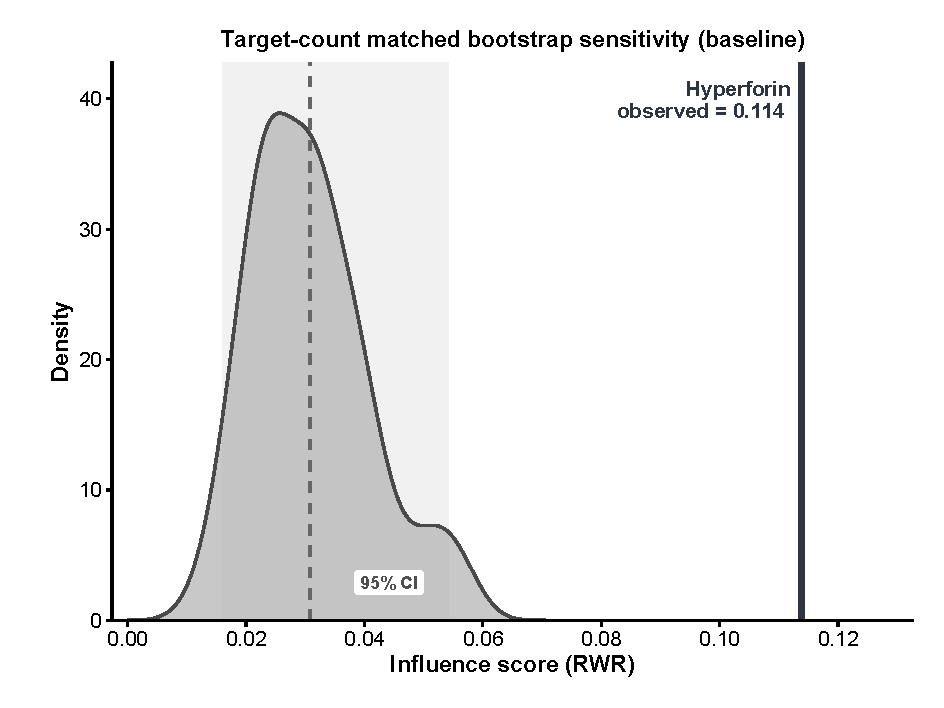
\includegraphics[width=0.7\textwidth]{figures/fig5_bootstrap.pdf}
\caption{\textbf{Bootstrap sensitivity (baseline).} Distribution of RWR influence for random 10-target subsets of Quercetin; solid line, Hyperforin observed influence. This baseline control does not adjust for target--DILI overlap; the leakage-controlled analysis (Table~\ref{tab:leakage}, Fig.~\ref{fig:leakage}) supersedes the headline ratio. STRING $\geq$900.}
\label{fig:bootstrap}
\end{figure}

\section*{Supplementary Tables}

% S1: Target-evidence table
\begin{table}[ht]
\centering
\caption{\textbf{Target curation evidence.} Hyperforin targets are literature-curated and span a direct nuclear receptor (PXR/NR1I2), PXR-induced downstream enzymes, transporters, and direct-inhibition targets; Quercetin targets are uniformly ChEMBL bioactivity-derived. This documents the evidentiary asymmetry whose downstream consequence is audited in Table~\ref{tab:s_leak}.}
\label{tab:s_evidence}
\small
\begin{tabular}{@{}llllccc@{}}
\toprule
\textbf{Gene} & \textbf{Source} & \textbf{Evidence type} & \textbf{Direct} & \textbf{In DILI} & \textbf{Shared} & \textbf{Kept$^\dagger$} \\
\midrule
\multicolumn{7}{l}{\textit{Hyperforin (literature-curated)}}\\
NR1I2  & literature & direct receptor agonist (PXR) & yes     & yes & no  & yes \\
CYP3A4 & literature & PXR-induced enzyme            & no      & no  & yes & no  \\
CYP2C9 & literature & enzyme (inhib./induction)     & partial & yes & no  & no  \\
CYP2B6 & literature & PXR-induced enzyme            & no      & no  & no  & no  \\
ABCB1  & literature & transporter (induced + inhib.)& yes     & yes & no  & no  \\
ABCG2  & literature & transporter modulation        & partial & no  & yes & no  \\
ABCC2  & literature & transporter modulation        & partial & no  & no  & no  \\
AKT1   & literature & direct kinase inhibition      & yes     & no  & yes & yes \\
MMP2   & literature & secretion inhibition          & partial & yes & yes & yes \\
MMP9   & literature & secretion inhibition          & partial & no  & yes & yes \\
\addlinespace
\multicolumn{7}{l}{\textit{Quercetin (ChEMBL bioactivity, CHEMBL159; 62 targets, full list Table~\ref{tab:s_quer})}}\\
\multicolumn{3}{l}{in vitro binding/activity (IC$_{50}$/K$_i$/EC$_{50}\leq$10\,$\mu$M)} & yes & MMP2 (1) & 5 & n/a \\
\bottomrule
\end{tabular}

\vspace{0.3em}
\begin{minipage}{\linewidth}\footnotesize ``Direct'' classifies the target--compound interaction: \textit{yes} = direct molecular target (receptor agonism or enzyme/kinase inhibition); \textit{partial} = mixed or context-dependent direct engagement (e.g.\ both induction and inhibition); \textit{no} = downstream induced effect rather than direct binding. $^\dagger$Kept = retained in the ``CYP/transporter-out'' leakage control (Table~\ref{tab:s_leak}).\end{minipage}
\end{table}

% S2: Hyperforin targets with CORRECTED degrees
\begin{table}[ht]
\centering
\caption{\textbf{Hyperforin targets in the liver-expressed LCC} (STRING $\geq$900). Node degrees are recomputed in the analysis network (correcting earlier values taken from a larger network). TPM from GTEx v8 liver.}
\label{tab:s_hyptargets}
\begin{tabular}{@{}llrrl@{}}
\toprule
\textbf{Gene} & \textbf{Protein} & \textbf{TPM} & \textbf{Degree} & \textbf{DILI link} \\
\midrule
NR1I2  & PXR         & 43  & 4   & direct (module member) \\
CYP3A4 & CYP3A4      & 335 & 73  & indirect \\
CYP2C9 & CYP2C9      & 434 & 52  & direct (module member) \\
CYP2B6 & CYP2B6      & 125 & 34  & indirect \\
AKT1   & PKB         & 33  & 128 & indirect \\
ABCB1  & P-gp        & 7   & 1   & direct (module member) \\
ABCC2  & MRP2        & 60  & 1   & indirect \\
ABCG2  & BCRP        & 4   & 2   & indirect \\
MMP2   & MMP-2       & 5   & 20  & direct (module member) \\
MMP9   & MMP-9       & 1   & 25  & indirect \\
\bottomrule
\end{tabular}
\end{table}

% (former null-SD-by-|T| table removed here: it duplicated main-text Table~2 verbatim;
%  the per-metric null parameters are tabulated below.)

% S-null: permutation null parameters by metric (Reviewer-2-referenced table)
\begin{table}[ht]
\centering
\caption{\textbf{Permutation null parameters across metrics} (STRING $\geq$900; $n=1{,}000$ degree-matched permutations). The null standard deviation $\sigma_{\text{null}}$ of the 62-target compound is $\approx$2.5$\times$ smaller than that of the 10-target compound for shortest-path, random-walk \emph{and} expression-weighted influence alike --- the Law-of-Large-Numbers shrinkage ($\sqrt{62/10}=2.49$), identical across metrics. This is why Z-score magnitude is not comparable across compounds of very different target count.}
\label{tab:s_nullsd}
\begin{tabular}{@{}ll S[table-format=1.4] S[table-format=1.4] S[table-format=1.4] S[table-format=+2.2]@{}}
\toprule
\textbf{Metric} & \textbf{Compound} & {$\mu_{\text{null}}$} & {$\sigma_{\text{null}}$} & {$x_{\text{obs}}$} & {$Z$} \\
\midrule
Shortest-path $d_c$ & Hyperforin (10) & 2.2086 & 0.2353 & 1.3000 & -3.86 \\
                    & Quercetin (62)  & 2.1749 & 0.0914 & 1.6774 & -5.44 \\
\addlinespace
RWR influence       & Hyperforin (10) & 0.0141 & 0.0093 & 0.1138 & +10.77 \\
                    & Quercetin (62)  & 0.0148 & 0.0038 & 0.0322 & +4.58 \\
\addlinespace
EWI influence       & Hyperforin (10) & 0.0196 & 0.0122 & 0.1330 & +9.28 \\
                    & Quercetin (62)  & 0.0210 & 0.0049 & 0.0493 & +5.74 \\
\midrule
\multicolumn{6}{@{}l}{\footnotesize $\sigma_{\text{null}}$ ratio (Hyperforin/Quercetin): shortest-path 2.57, RWR 2.45, EWI 2.47 (expected $\sqrt{62/10}=2.49$).}\\
\bottomrule
\end{tabular}
\end{table}

% S-opregime: operating-regime reversal rates
\begin{table}[ht]
\centering
\caption{\textbf{Operating-regime benchmark: margin-conditional rank-reversal rates} (liver LCC $\geq$900, DILI module; probes pinned to the full compound-target row degree profile, with DILI-module genes excluded from the candidate pool; smaller set $|T_S|=10$; $500{,}000$ probe pairs per row, seed 42). Each entry is the fraction of pairs in which the smaller set is genuinely closer by a material raw margin ($\geq\delta_0$ hops) yet the larger set has the more negative Z-score. Reversals are rare and require a smaller set above the 90th percentile of probe-pair margins: a no-shrinkage counterfactual ($\sigma_L:=\sigma_S$) gives $0\%$ at every $R$, and unconditionally the Hyperforin/Quercetin directional pattern (smaller set closer \emph{and} larger set stronger Z) occurs in only $6.5\%$ of exact $R=6.2$ pairs, collapsing to near-zero once a material margin is required. The null-SD exponent is $-0.499$ (95\% CI $[-0.502,-0.495]$, $R^2=0.9999$) and similar across the DILI module and three size-matched pseudo-modules (DILI $-0.495$; three random size-matched pseudo-modules mean $-0.498$).}
\label{tab:s_opregime}
\begin{tabular}{@{}cc S[table-format=1.2] S[table-format=1.2]@{}}
\toprule
$R=|T_L|/|T_S|$ & $(|T_S|,|T_L|)$ & {reversal, $\delta_0\geq0.3$ (\%)} & {reversal, $\delta_0\geq0.5$ (\%)} \\
\midrule
1.5 & (10,\,15) & 0.00 & 0.00 \\
2.0 & (10,\,20) & 0.00 & 0.00 \\
3.0 & (10,\,30) & 0.00 & 0.00 \\
4.0 & (10,\,40) & 0.00 & 0.00 \\
6.0 & (10,\,60) & 0.10 & 0.00 \\
6.2 & (10,\,62) & 0.06 & 0.00 \\
8.0 & (10,\,80) & 0.39 & 0.00 \\
\bottomrule
\end{tabular}
\end{table}

% S-textmining: text-mining sensitivity values (before/after removing TM-only edges)
\begin{table}[ht]
\centering
\caption{\textbf{Text-mining robustness: metric values before and after removing text-mining-only STRING edges} (liver-expressed LCC; following \citet{Huang2018}, every edge supported \textit{solely} by the STRING text-mining channel was removed). ``Committed'' is the value in the main analysis; ``no-TM'' is after removal. The Hyperforin\,$>$\,Quercetin ordering (smaller $d_c$; larger influence) is preserved on all three metrics at both network thresholds, and every no-TM permutation $p<0.002$; arguing against literature text-mining circularity as the driver. Source: \texttt{results/tables/string\_textmining\_sensitivity.csv}.}
\label{tab:s_textmining}
\small
\begin{tabular}{@{}ll S[table-format=1.4] S[table-format=1.4] S[table-format=1.4] S[table-format=1.4] c@{}}
\toprule
& & \multicolumn{2}{c}{\textbf{Hyperforin}} & \multicolumn{2}{c}{\textbf{Quercetin}} & \\
\cmidrule(lr){3-4}\cmidrule(lr){5-6}
\textbf{Metric} & \textbf{STRING} & {committed} & {no-TM} & {committed} & {no-TM} & \textbf{winner} \\
\midrule
$d_c$ (smaller closer) & $\geq$700 & 0.6000 & 0.6000 & 1.3387 & 1.3387 & Hyp \\
                       & $\geq$900 & 1.3000 & 1.3000 & 1.6774 & 1.6721 & Hyp \\
\addlinespace
RWR influence (larger) & $\geq$700 & 0.1212 & 0.1243 & 0.0326 & 0.0335 & Hyp \\
                       & $\geq$900 & 0.1138 & 0.1144 & 0.0322 & 0.0329 & Hyp \\
\addlinespace
EWI influence (larger) & $\geq$700 & 0.1449 & 0.1472 & 0.0511 & 0.0516 & Hyp \\
                       & $\geq$900 & 0.1330 & 0.1337 & 0.0493 & 0.0501 & Hyp \\
\bottomrule
\end{tabular}
\end{table}

% S4: threshold robustness (>=700 vs >=900)
\begin{table}[ht]
\centering
\caption{\textbf{Threshold robustness} (STRING $\geq$700 vs $\geq$900 liver LCC; $n=1{,}000$, seed 42). The proximity-Z \emph{ranking} reverses across thresholds --- Hyperforin is the more ``significant'' at $\geq$700, Quercetin at $\geq$900 --- whereas the raw closest distance ($d_c$, Hyperforin closer) and the per-target influence ($E$, Hyperforin higher) rankings are stable at both thresholds. This is the effect-size/evidence dissociation of the main text, shown across network construction.}
\label{tab:s_threshold}
\begin{tabular}{@{}llcccc@{}}
\toprule
& & \multicolumn{2}{c}{\textbf{STRING $\geq$700}} & \multicolumn{2}{c}{\textbf{STRING $\geq$900}} \\
\cmidrule(lr){3-4}\cmidrule(lr){5-6}
\textbf{Metric} & \textbf{Compound} & value & $Z$ & value & $Z$ \\
\midrule
$d_c$ (closest distance) & Hyperforin & 0.60 & $-6.04$ & 1.30 & $-3.86$ \\
                         & Quercetin  & 1.34 & $-5.46$ & 1.68 & $-5.44$ \\
\addlinespace
$E$ (RWR influence)      & Hyperforin & 0.1212 & $+11.04$ & 0.1138 & $+10.77$ \\
                         & Quercetin  & 0.0326 & $+5.46$  & 0.0322 & $+4.58$ \\
\addlinespace
$E$ (EWI influence)      & Hyperforin & 0.1449 & $+10.35$ & 0.1330 & $+9.28$ \\
                         & Quercetin  & 0.0511 & $+7.01$  & 0.0493 & $+5.74$ \\
\bottomrule
\end{tabular}
\end{table}

% S5: alpha sweep
\begin{table}[ht]
\centering
\caption{\textbf{Restart-probability ($\alpha$) sensitivity} (STRING $\geq$900). The Hyperforin $>$ Quercetin per-target-efficiency ranking holds at every $\alpha$; the ratio is $\alpha$-dependent and is not interpreted as an absolute constant.}
\label{tab:s_alpha}
\begin{tabular}{@{}lcccccc@{}}
\toprule
$\alpha$ & 0.10 & 0.15 & 0.20 & 0.30 & 0.50 & 0.70 \\
\midrule
$E$ Hyperforin & 0.0907 & 0.1138 & 0.1344 & 0.1716 & 0.2390 & 0.3032 \\
$E$ Quercetin  & 0.0312 & 0.0322 & 0.0322 & 0.0310 & 0.0271 & 0.0227 \\
ratio          & 2.90 & 3.54 & 4.18 & 5.53 & 8.81 & 13.35 \\
\bottomrule
\end{tabular}
\end{table}

% S5: floor sweep
\begin{table}[ht]
\centering
\caption{\textbf{Expression-floor sensitivity (EWI)} (STRING $\geq$900). The 0.01 floor is immaterial; the ratio moves only in the third decimal.}
\label{tab:s_floor}
\begin{tabular}{@{}lccccc@{}}
\toprule
floor & 0 & $10^{-3}$ & $10^{-2}$ & $5\times10^{-2}$ & $10^{-1}$ \\
\midrule
$E$ Hyperforin & 0.1330 & 0.1330 & 0.1330 & 0.1330 & 0.1327 \\
$E$ Quercetin  & 0.0493 & 0.0493 & 0.0493 & 0.0493 & 0.0491 \\
ratio          & 2.695 & 2.695 & 2.695 & 2.695 & 2.702 \\
\bottomrule
\end{tabular}
\end{table}

% S6: direct-propagated decomposition (full controls)
\begin{table}[ht]
\centering
\caption{\textbf{Direct--propagated decomposition of per-target influence: full controls} (STRING $\geq$900). Four of ten Hyperforin targets are DILI-module members vs one of 62 Quercetin targets; isolating the propagated component (leave-one-out) and removing each source of direct overlap attenuates the per-target advantage to a modest residual.}
\label{tab:s_leak}
\begin{tabular}{@{}p{0.36\textwidth}ccc@{}}
\toprule
\textbf{Control} & \textbf{$E$(Hyp)} & \textbf{$E$(Quer)} & \textbf{ratio} \\
\midrule
Baseline (includes overlap) & 0.1138 & 0.0322 & 3.54 \\
Self-mass excluded & 0.0427 & 0.0290 & 1.47 \\
DILI-member seeds removed & 0.0431 & 0.0295 & 1.46 \\
CYP/transporter seeds removed & 0.0338 & 0.0290 & 1.17 \\
Shared targets removed (both) & 0.0541 & 0.0288 & 1.88 \\
\midrule
\multicolumn{4}{@{}p{0.95\textwidth}@{}}{\textit{Propagated (leave-one-out) reference distributions ($n=1{,}000$; Fig.~\ref{fig:leakage}B):}}\\
Global degree-matched random set ($n=10$) & \multicolumn{3}{p{0.52\textwidth}@{}}{Hyp 0.0427 vs null mean 0.0130 (95th 0.0281; max 0.0580); 99.9th percentile, 3.3$\times$ mean, $p=0.002$, does not exceed all}\\
Size-matched Quercetin 10-subsets & \multicolumn{3}{p{0.52\textwidth}@{}}{Hyp 0.0427 vs subset mean 0.0296 (max 0.0622); 1.4$\times$, overlapping}\\
\bottomrule
\end{tabular}
\end{table}

% S7: separation measure (Menche 2015)
\begin{table}[ht]
\centering
\caption{\textbf{Network separation between target set and DILI module.} Menche et al.\ separation measure $S_{AB}=\langle d_{AB}\rangle-(\langle d_{AA}\rangle+\langle d_{BB}\rangle)/2$ \citep{Menche2015} (STRING $\geq$900); $S_{AB}>0$ indicates topological separation. Both target sets are separated from the DILI module, and Hyperforin is \emph{more} separated despite its four direct-overlap targets, because its targets form a tighter cluster ($\langle d_{AA}\rangle=1.20$ vs $1.55$). This corroborates the decomposition (Table~\ref{tab:leakage}, Fig.~\ref{fig:leakage}): Hyperforin's per-target influence advantage arises from a few targets that \emph{are} DILI genes (direct overlap), not from its target set being embedded in the DILI neighbourhood.}
\label{tab:s_sep}
\begin{tabular}{@{}l S[table-format=1.3] S[table-format=1.3] S[table-format=1.3] S[table-format=+1.3]@{}}
\toprule
\textbf{Target set} & {$\langle d_{AB}\rangle$} & {$\langle d_{AA}\rangle$} & {$\langle d_{BB}\rangle$} & {$S_{AB}$} \\
\midrule
Hyperforin & 1.699 & 1.200 & 1.500 & +0.349 \\
Quercetin  & 1.644 & 1.548 & 1.500 & +0.119 \\
\bottomrule
\end{tabular}
\end{table}

% S-connectivity: direct (distance-1) DILI connectivity (regenerated on >=900 LCC)
\begin{table}[ht]
\centering
\caption{\textbf{Direct (distance-1) DILI connectivity of Hyperforin targets} (regenerated on the STRING $\geq$900 liver LCC). Connectivity is concentrated in the cytochrome-P450 axis; the transporters (ABCB1, ABCC2, ABCG2) and the receptor NR1I2 have no additional distance-1 DILI neighbours (NR1I2 and ABCB1 are themselves module members, at distance 0). Per-target means: \textbf{Hyperforin 3.40} direct DILI neighbours (34 connections across 10 targets) vs \textbf{Quercetin 1.53} (95 across 62) --- a $2.2\times$ enrichment that complements the distance-0 direct-overlap decomposition (Table~\ref{tab:s_leak}).}
\label{tab:s_connectivity}
\footnotesize
\begin{tabular}{@{}lcp{9.4cm}@{}}
\toprule
\textbf{Hyperforin target} & \textbf{$n$} & \textbf{Direct DILI neighbours (distance 1)} \\
\midrule
CYP3A4 & 11 & CYP2A6, CYP2C19, CYP2C9, CYP2E1, FMO3, GSTM1, GSTM2, GSTP1, NR1I2, NR1I3, UGT1A9 \\
CYP2C9 & 9  & CYP2A6, CYP2C19, CYP2E1, FMO3, GSTM1, GSTM2, GSTP1, PTGS2, UGT1A9 \\
CYP2B6 & 6  & CYP2A6, CYP2C19, CYP2C9, CYP2E1, PTGS2, UGT1A9 \\
AKT1   & 4  & CTNNB1, IGF1, MAP3K5, NFE2L2 \\
MMP9   & 3  & LCN2, MMP2, SPP1 \\
MMP2   & 1  & LCN2 \\
ABCB1, ABCC2, ABCG2, NR1I2 & 0 & --- \\
\bottomrule
\end{tabular}
\end{table}

% S-modulesens: DILI-module sensitivity (remove entangled pharmacogenes from the module)
\begin{table}[ht]
\centering
\caption{\textbf{DILI-module sensitivity: removing the entangled pharmacogenes.} Every other robustness check in this work varies the \emph{method} ($\alpha$, expression floor, network threshold, degree-binning, two nulls); this one varies the \emph{disease module}, the locus of the target--disease circularity. We remove from the 82-gene module the four genes that are simultaneously Hyperforin targets and DILI members (ABCB1, CYP2C9, MMP2, NR1I2), giving a reduced module $D'$ that the drug targets cannot directly overlap, and recompute the propagated (leave-one-out) per-target influence symmetrically for both compounds (STRING $\geq$900, $\alpha=0.15$). The propagated advantage does \emph{not} collapse --- it slightly increases, because Hyperforin's leave-one-out value is unchanged (those genes were already excluded from its own scoring) while Quercetin loses propagation onto ABCB1/CYP2C9/NR1I2, which it had benefited from as non-target DILI genes. Against a degree-matched random 10-gene background scored on $D'$ ($n=1{,}000$), Hyperforin remains at the 99th percentile ($3.45\times$ the background mean, empirical $p=0.005$) but does not exceed every random set. The modest propagated signal supports the interpretation that the propagated residual is not eliminated after removing the overlapping pharmacogenes from the module.}
\label{tab:s_modulesens}
\begin{tabular}{@{}l S[table-format=2.0] S[table-format=1.4] S[table-format=1.4] S[table-format=1.2]@{}}
\toprule
\textbf{Disease module} & {$|D|$} & {Propagated $E$ (Hyp)} & {Propagated $E$ (Quer)} & {Ratio} \\
\midrule
Full DILI module            & 82 & 0.0427 & 0.0290 & 1.47 \\
Overlap genes removed ($D'$) & 78 & 0.0427 & 0.0271 & 1.58 \\
\bottomrule
\end{tabular}
\end{table}

% S10: Guney fidelity -- full null parameters (expanded companion to main-text Table tab:guney)
\begin{table}[ht]
\centering
\caption{\textbf{Independent reimplementation of the canonical proximity toolbox: full null parameters} (\texttt{emreg00/toolbox}, re-derived by \texttt{GUNEY\_FIDELITY\_check.py}; STRING $\geq$900; $n=1{,}000$; seed 42; $|D|=82$ preserved). This is the detailed companion to the compact main-text summary (Table~\ref{tab:guney}): for each null construction it reports the observed closest distance $d_c$, the null mean $\mu_{\text{null}}$ and standard deviation $\sigma_{\text{null}}$, and the resulting $Z$. The observed $d_c$ reproduces the toolbox exactly (Hyperforin 1.300, Quercetin 1.677). The reimplementation's $\pm$25\% window (group 1, Quercetin $Z=-5.35$) matches the committed \texttt{src} pipeline ($Z=-5.44$; Table~\ref{tab:s_nullsd}) within permutation tolerance, confirming the two implementations agree. The $\pm$25\% window never silently falls back to unmatched nodes: every Hyperforin target retains $\geq$143 degree-matched candidates (its highest-degree target, AKT1, has degree 128). The evidence dissociation is clear under the fixed-disease null and attenuates to near-parity under the two-sided null; Hyperforin is the topologically closer compound throughout.}
\label{tab:s_guney}
\begin{tabular}{@{}ll S[table-format=1.2] S[table-format=1.2] S[table-format=1.3] S[table-format=-1.2]@{}}
\toprule
\textbf{Null model} & \textbf{Compound} & {$d_c$} & {$\mu_{\text{null}}$} & {$\sigma_{\text{null}}$} & {$Z$} \\
\midrule
$\pm$25\% window, fixed disease & Hyperforin & 1.30 & 2.22 & 0.238 & -3.86 \\
                                & Quercetin  & 1.68 & 2.18 & 0.093 & -5.35 \\
\addlinespace
Guney $\geq$100-bin, fixed disease & Hyperforin & 1.30 & 2.23 & 0.228 & -4.09 \\
                                   & Quercetin  & 1.68 & 2.16 & 0.090 & -5.34 \\
\addlinespace
Guney $\geq$100-bin, two-sided & Hyperforin & 1.30 & 2.05 & 0.212 & -3.55 \\
                               & Quercetin  & 1.68 & 2.01 & 0.090 & -3.66 \\
\midrule
\multicolumn{6}{@{}p{0.92\textwidth}}{\footnotesize $\sigma_{\text{null}}$ ratio (Hyperforin/Quercetin), from full-precision values: 2.56 ($\pm$25\% fixed), 2.53 ($\geq$100-bin fixed), 2.37 ($\geq$100-bin two-sided); expected $\sqrt{62/10}=2.49$. The Law-of-Large-Numbers shrinkage therefore persists under every null construction, including Guney's exact two-sided null.}\\
\bottomrule
\end{tabular}
\end{table}

% S8: full Quercetin list
\begin{table}[ht]
\centering
\caption{\textbf{Quercetin target genes in the liver-expressed LCC} (STRING $\geq$900, GTEx v8 liver TPM $\geq$1; ChEMBL CHEMBL159). Sorted by descending TPM.}
\label{tab:s_quer}
\scriptsize
\begin{tabular}{lrlrlrlr}
\toprule
\textbf{Gene} & \textbf{TPM} & \textbf{Gene} & \textbf{TPM} & \textbf{Gene} & \textbf{TPM} & \textbf{Gene} & \textbf{TPM} \\
\midrule
CFB & 1115 & CYP3A4 & 335 & FN1 & 229 & ALDH2 & 183 \\
ANPEP & 160 & PPIA & 112 & SERPINA5 & 104 & CYP1A2 & 72 \\
CA2 & 64 & APP & 63 & PYGL & 55 & HDAC6 & 45 \\
ESRRA & 42 & MAOA & 35 & AKR1C2 & 33 & AKT1 & 33 \\
CTSH & 28 & XDH & 26 & CHRNA4 & 25 & PIK3R1 & 24 \\
PIM1 & 24 & LDLR & 23 & ELOVL1 & 18 & EGFR & 17 \\
PKN1 & 16 & GSK3A & 13 & YES1 & 13 & MET & 12 \\
DAPK1 & 12 & BACE1 & 11 & CSNK2A1 & 10 & FSTL1 & 9 \\
SIRT6 & 8 & GSK3B & 7 & CDK7 & 7 & CAV2 & 7 \\
PTPN2 & 6 & CYP1A1 & 5 & PRMT7 & 5 & MMP2 & 5 \\
AKR1B1 & 5 & PDE6D & 5 & BRAF & 4 & PTK2 & 4 \\
ABCG2 & 4 & IQGAP1 & 4 & ADRB2 & 3 & KDR & 3 \\
SRC & 3 & ALOX5 & 3 & CYP1B1 & 3 & TLR4 & 3 \\
NUAK1 & 3 & AXL & 2 & ADA & 2 & LCK & 2 \\
ABCC1 & 2 & PLK1 & 1 & ACHE & 1 & MMP9 & 1 \\
SYK & 1 & PDZK1IP1 & 1 & & & & \\
\bottomrule
\end{tabular}
\end{table}

% S-curation: curation provenance
\begin{table}[ht]
\centering
\caption{\textbf{Curation provenance} (stage counts, reproducible from the committed data). Targets are filtered to the intersection of the $\geq$700 and $\geq$900 liver LCCs, so target counts are identical at both thresholds; the DILI module is filtered per threshold.}
\label{tab:s_curation}
\begin{tabular}{@{}lrrr@{}}
\toprule
\textbf{Stage} & \textbf{Hyperforin} & \textbf{Quercetin} & \textbf{DILI module} \\
\midrule
Raw (lit. / ChEMBL / DisGeNET) & 14 & 122 & 127 \\
Processed (human, UniProt-mapped)              & 14 & 87  & --- \\
In $\geq$700 liver-expressed LCC               & 10 & 62  & 84 \\
In $\geq$900 liver-expressed LCC               & 10 & 62  & 82 \\
\bottomrule
\end{tabular}
\end{table}

% S-dili: full DILI gene list
\begin{table}[ht]
\centering
\caption{\textbf{DILI gene set (82 genes)} in the liver-expressed STRING $\geq$900 LCC (DisGeNET, UMLS C0860207; GTEx v8 liver TPM $\geq$1), alphabetical. The four genes that are also Hyperforin targets (the distance-0 direct overlap, Table~\ref{tab:s_leak}) are in bold.}
\label{tab:s_dili}
\scriptsize
\begin{tabular}{llllllll}
\toprule
\multicolumn{8}{c}{\textbf{82 DILI-associated genes}} \\
\midrule
\textbf{ABCB1} & AHR & ALB & ALDOB & AMBP & APOA1 & APOE & APOH \\
ARG1 & ARNT & ATG5 & BAX & BTD & C3 & CAT & CCL2 \\
CLU & COL3A1 & CTNNB1 & CXCL1 & CXCL10 & CYP2A6 & CYP2C19 & \textbf{CYP2C9} \\
CYP2E1 & DGAT2 & ENO1 & FGA & FLT1 & FMO3 & GADD45A & GC \\
GCLC & GPT & GSN & GSTM1 & GSTM2 & GSTP1 & HLA-A & HLA-B \\
HLA-DQB1 & HLA-DRB1 & HMGB1 & HMOX1 & HPD & HPX & IGF1 & IL18 \\
IL1R2 & KRT18 & LCN2 & LGALS3 & MAP3K5 & MED1 & \textbf{MMP2} & MTHFR \\
NAT2 & NFE2L2 & NR1H3 & NR1H4 & \textbf{NR1I2} & NR1I3 & PLAT & PLG \\
PNP & POLG & PON1 & PPARA & PRKDC & PTGS2 & RBP1 & SLPI \\
SNX18 & SOD1 & SOD3 & SPP1 & TALDO1 & TBXA2R & TCTN1 & TF \\
TTR & UGT1A9 & & & & & & \\
\bottomrule
\end{tabular}
\end{table}

\noindent\footnotesize All values above are regenerated by the committed pipeline and reviewer-evidence scripts; cross-document numerical consistency is enforced by \texttt{verify\_numbers.py}.
